\begin{frame} \frametitle{US pulse and Trapezoidal acoustic waveforms are used.}
  \begin{figure}
    \centering
    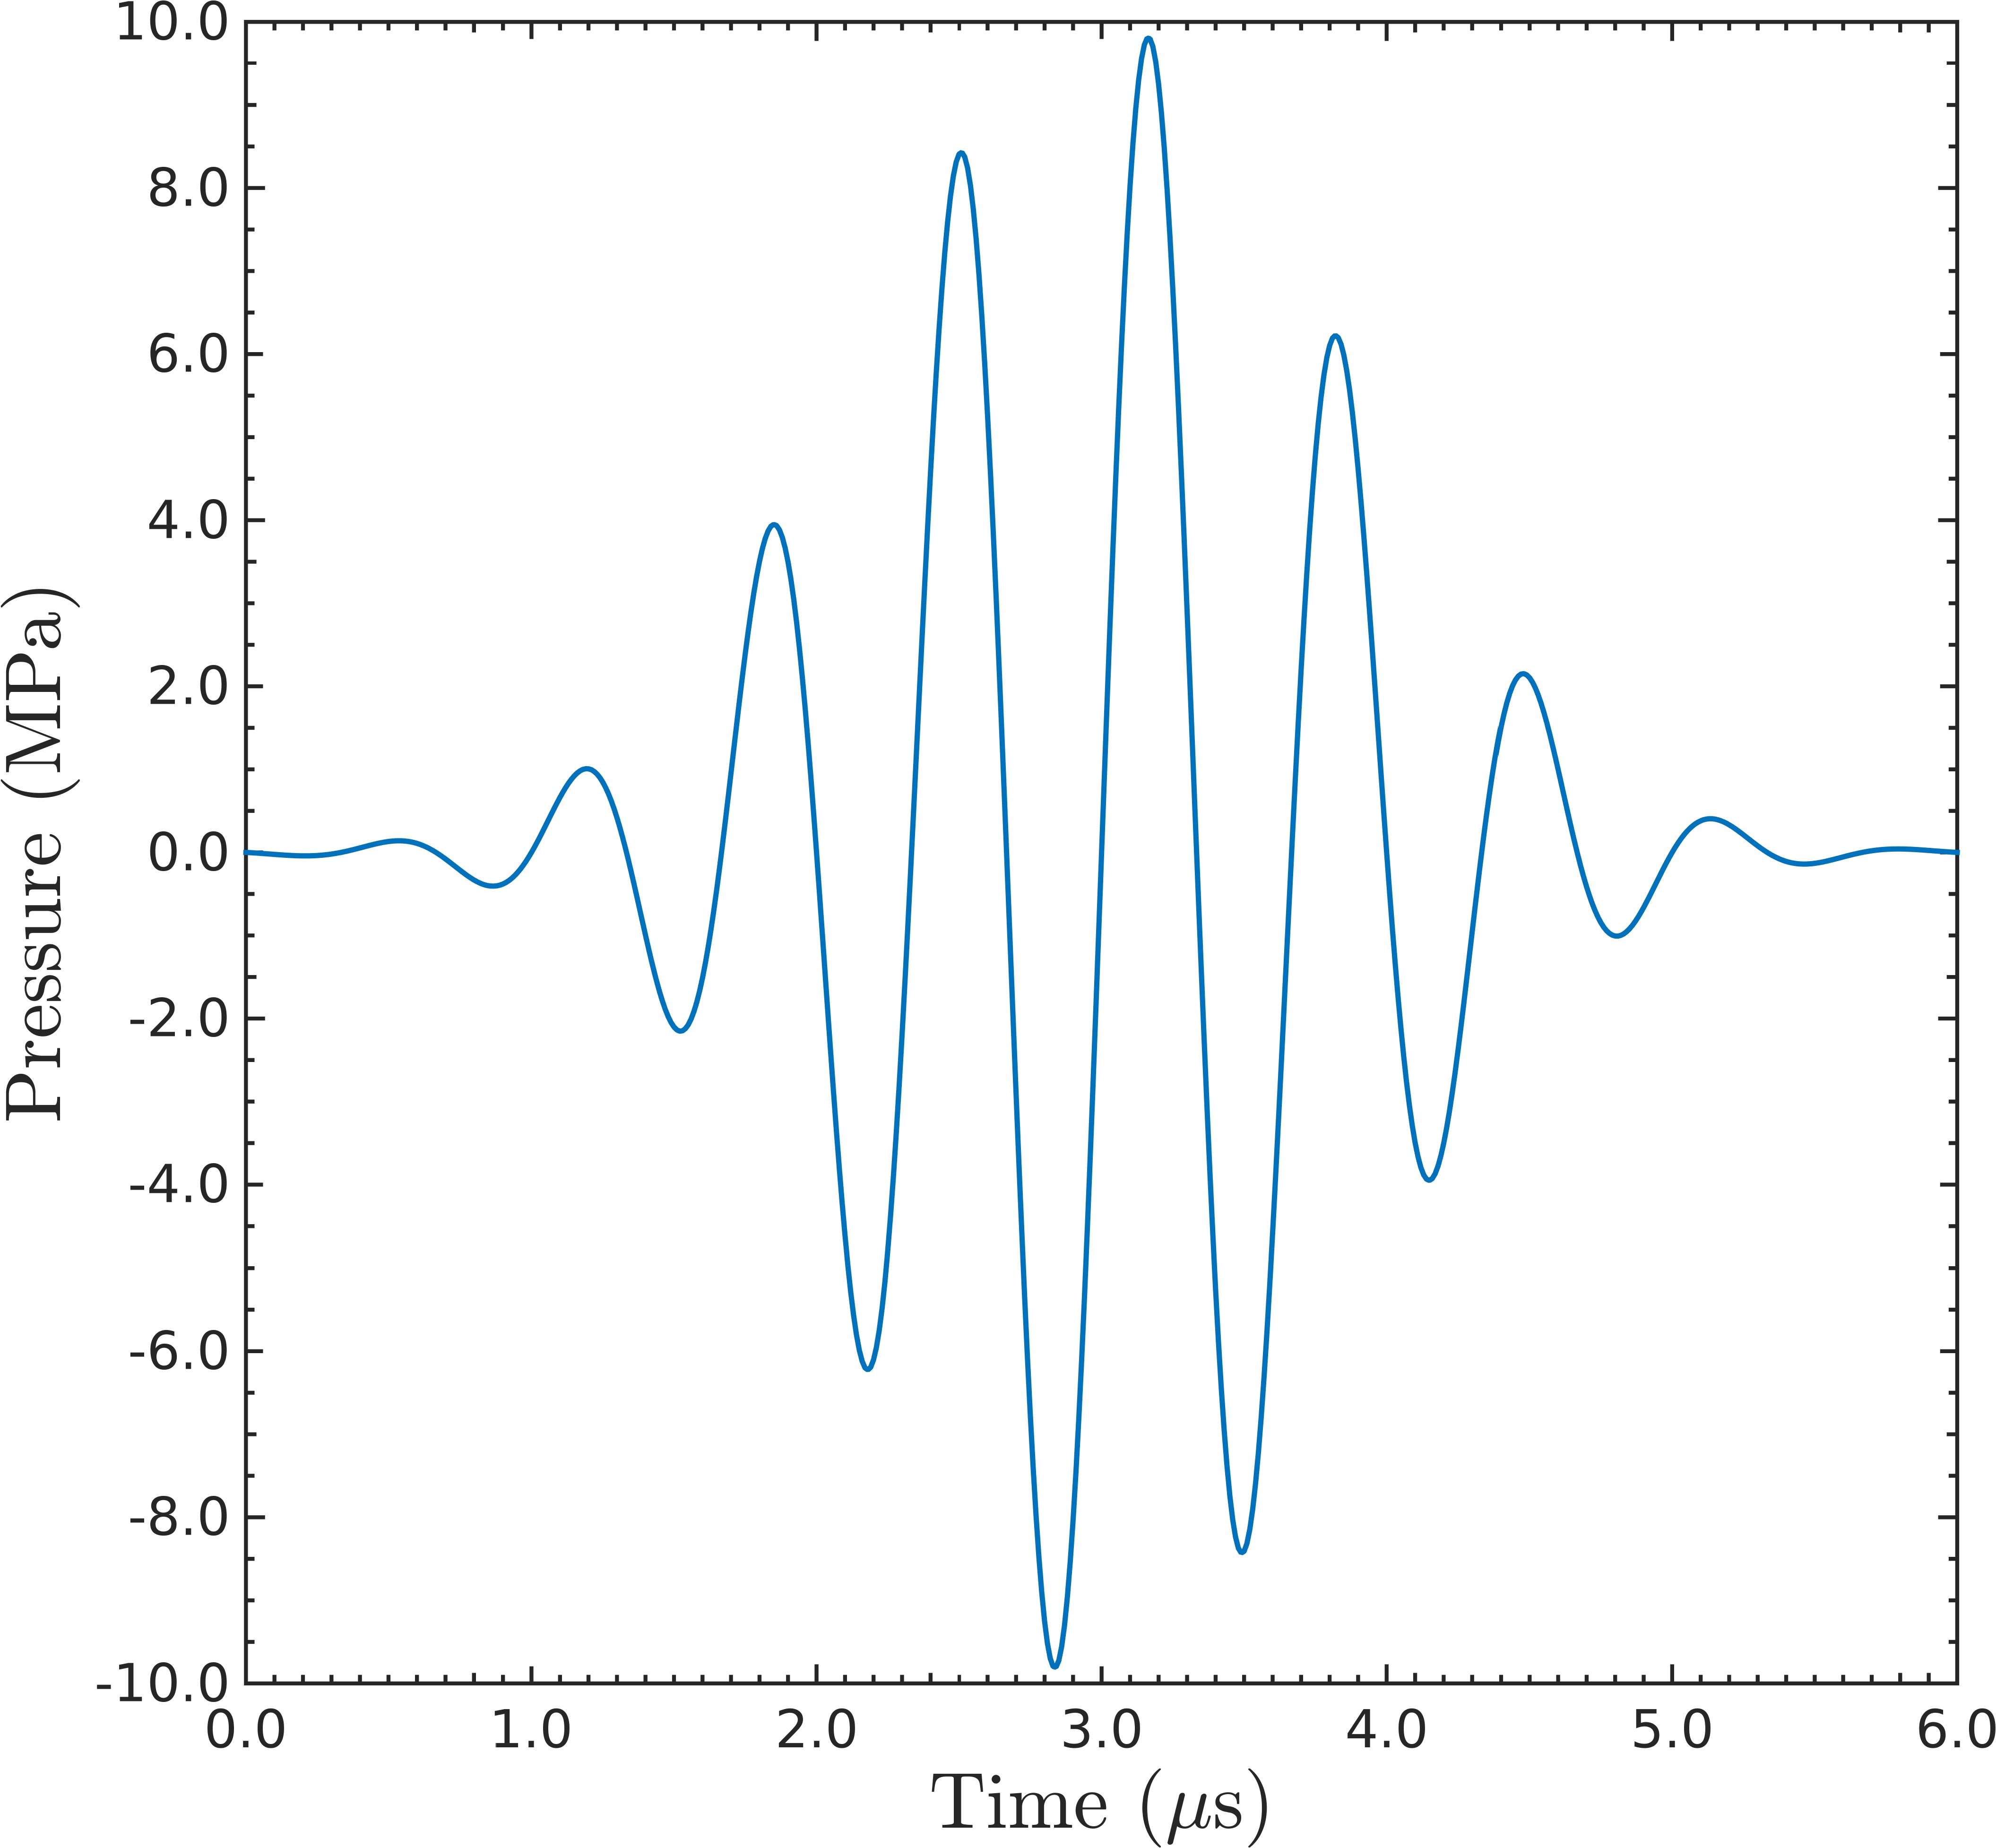
\includegraphics[height=0.4\textheight]{../figs/lung_figs/p0_vs_t_us}\hfill%
    \visible<2->{
    \def\svgwidth{0.25\textwidth}
      {\footnotesize
        \import{../figs/lung_figs/}{wave_logic_schematic2.pdf_tex}%
      }
    }
    \hfill%
    \visible<3->{
    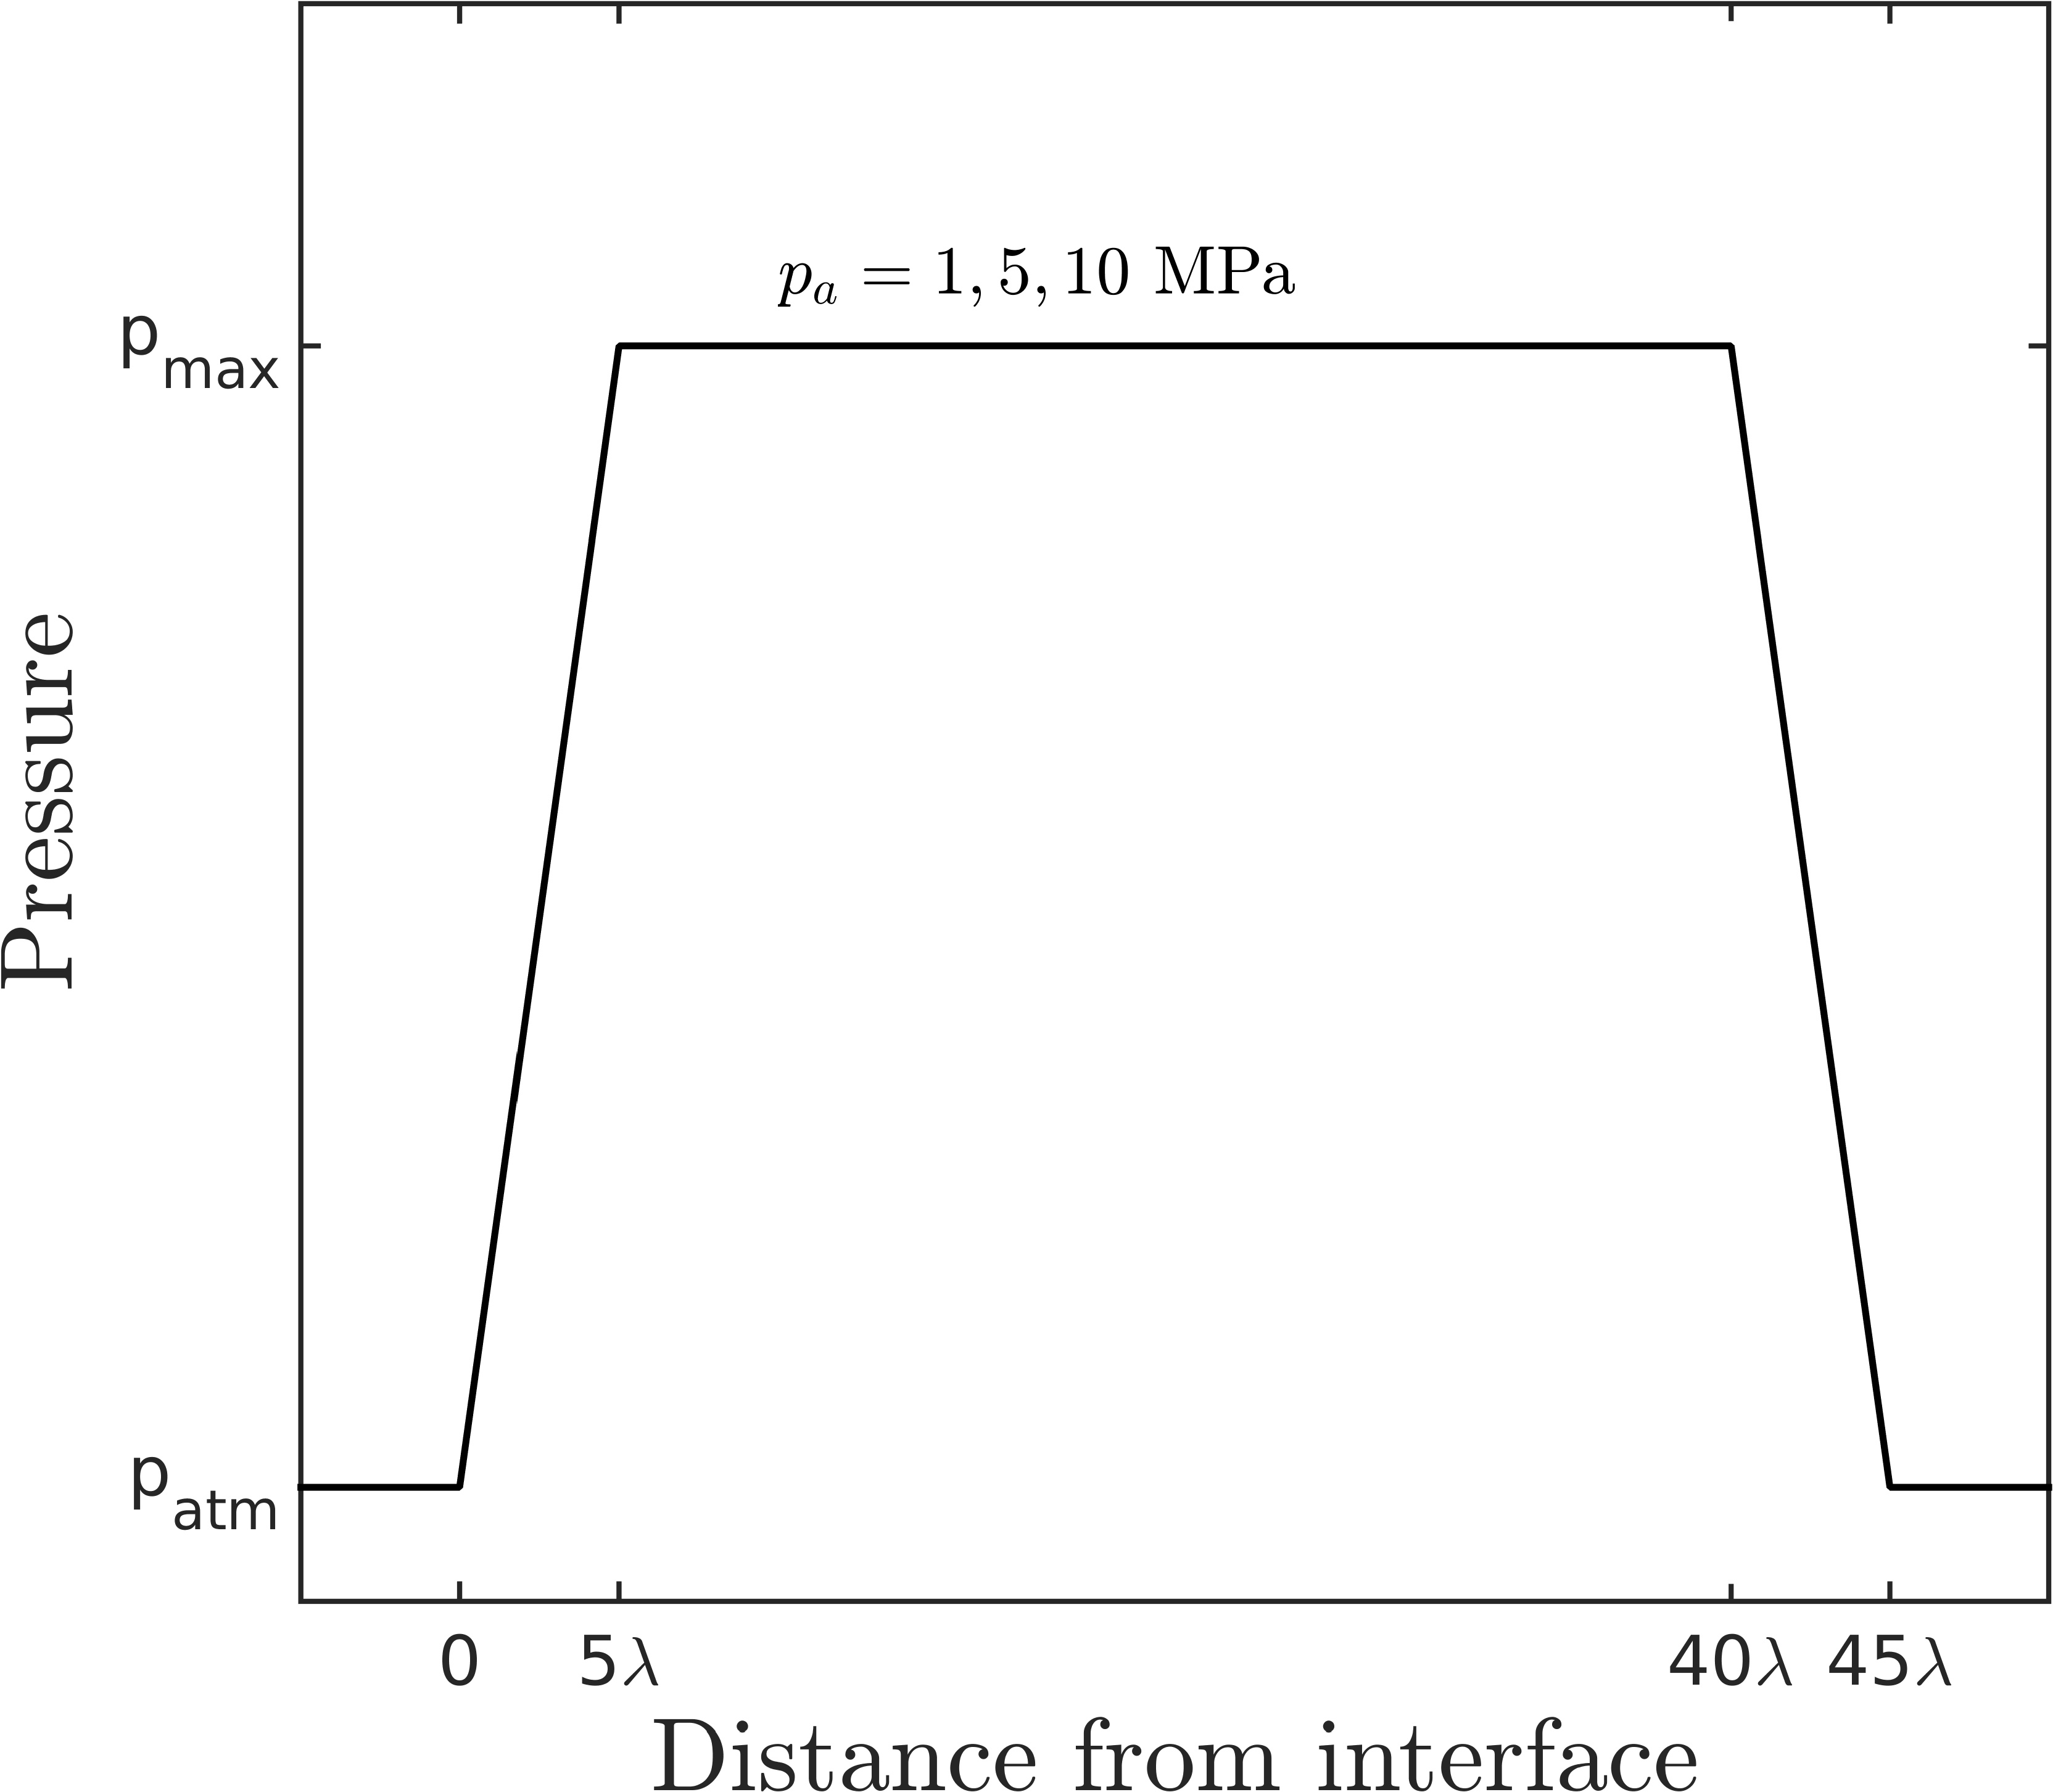
\includegraphics[height=0.4\textheight]{../figs/lung_figs/p0_vs_y}%
    }
  \end{figure}
  \visible<3->{
    \begin{itemize}
    \item The trapezoidal waves is simple for understanding physics and analysis, but able to capture feature of US pulse.
    \item Pulse waveforms are used to check relevance to DUS.
    \end{itemize}
  }
\end{frame}
%%% Local Variables:
%%% mode: latex
%%% TeX-master: "../main"
%%% End:
